\chapter{Коллективная азимутальная анизотропия в столкновениях тяжелых ионов} \label{chapt1}

\section{Обзор литературы по столкновениям тяжелых ионов}

\subsection{Уравнение состояния и фазовая диаграмма КХД материи}

Равновесные свойства сильновзаимодействующей материи выражаются в форме уравнения состояния (Equation Of State — EOS). 
Уравнение состояния определяет взаимосвязь между макроскопическими характеристиками материи, такими как температура, плотность, вязкость, давление и другие.
В современных моделях сильновзаимодействующей материи, основанных на гидродинамическом или статистическом подходах, уравнение состояния играет ключевую роль.
Фазовое состояние сильно взаимодействующей материи зависит от температуры ($T$) и бариохимического потенциала ($\mu_B$).
Фазовая диаграмма сильновзаимодействующей материи представлена на рис.~\ref{fig:qcd_phase_diagram}~\cite{Bzdak:2019pkr}.
%
\begin{figure}[h]
    \centering
    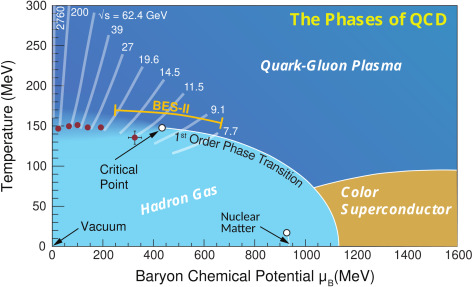
\includegraphics[width=0.5\linewidth]{images/1-s2.0-S0370157320300156-gr1.jpg}
    \caption{Фазовая диаграмма КХД-материи~\cite{Bzdak:2019pkr}.}
    \label{fig:qcd_phase_diagram}
\end{figure}

При больших температурах и низких бариохимических потенциалах, сильновзаимодействующая материя проявляет партонные степени свободы и характеризуется деконфайнментом кварков. 
Открытое в 2005 году на релятивистском ускорителе тяжелых RHIC~\cite{STAR:2005gfr}, это состояние получило название кварк-глюонной плазмы КГП.
Исследуя коллективные потоки, рожденных в столкновениях тяжелых ионов, было установлено, что эта форма материи обладает наименьшей известной в природе сдвиговой вязкостью.~\cite{Shen:2015msa}.
Вычисления КХД на решетке предсказывают плавный переход типа "crossover" от партонных степеней своды к адронным, при низких бариохимических потенциалах с уменьшением температуры~\cite{HotQCD:2014kol, Karsch:2003va}.
Экспериментальные доказательства этому были обнаружены в ходе первого скана по энергии на RHIC~\cite{Odyniec:2019kfh}.
Согласно современным представлениям, эпохе бариогенезиса предшествовало состояние горячей КГП с около нулевым барионным числом, которое завершилось плавным "crossover" переходом в состояние материи с преимущественно адронными степенями свободы~\cite{Esumi:2022uas}

При ненулевых бариохимических потенциалах, КХД-расчеты предсказывают переход первого рода из состояния с адронными степенями свободы в состояние с преимущественно кварковыми.
Существование двух видов фазового перехода: плавный типа "crossover" и перехода первого рода в одной области бариохимических потенциалов и температуры предполагает наличие критической точки~\cite{Odyniec:2019kfh}.
В области невысоких теператур и сверхвысоких бариохимических потенциалов теоретически предсказано существование еще более экзотической формы материи, такой как цвето-сверхпроводящая материя~\cite{McLerran:2008ux}.

В столкновениях тяжелых ионов при кинетических энергиях в несколько $A$~ГэВ образуется сильновзаимодействующая материя при температурах $T\approx150$~МэВ и чистых барионных плотностях в несколько раз превышающих плотность ядреной материи.
Исследование этой области фазовой диаграммы представляет интерес, поскольку предполагается, что такая материя встречается в компактных астрофизических объектах, к примеру, в нейтронных звёздах~\cite{Danielewicz:2002pu}.
Столкновениях ионов --- единственный способ лабораторно воссоздать условия, существующие в сложнонаблюдаемых космологических объектах.

Направленный и эллиптический потоки являются чувствительными наблюдаемыми к уравнению состояния, поскольку отражают изначальное распределение градиентов давления в системе.
Вычисления релятивистской гидродинамики предсказывают, что "смягчение" уравнения состояния должно сильно влиять на магнитуду и знак направленного потока протонов, что может являться сигналом фазового перехода первого рода при высоких барионных плотностях~\cite{Rischke:1995pe, Stoecker:2004qu}.
С ростом энергии и смягчении уравнения состояния, направленный поток должен менять знак с положительно на отрицательный.
Такая зависимость от энергии действительно наблюдалась в данных, опубликованных коллаборацией STAR~\cite{STAR:2014clz}.

\subsection{Описание динамики столкновения тяжелых ионов}


В результате столкновения тяжелых ионов в области перекрытия образуется сильно взаимодействующая материя, свойства которой сильно зависят от размера сталкивающихся ядер, и от энергии столкновения.
При столкновении тяжелых ядер, при энергиях в несколько ГэВ на нуклон налетающего ядра, время пролёта ионов сравнимо со временем существования материи в области перекрытия.
Процесс столкновения двух ядер можно условно разделить на несколько этапов.

При скоростях налетающего ядра, превышающих скорость звука в ядерной материи при обычных условиях ($\beta_S=0.2$)~\cite{Weber:1998aa}, нуклоны не могут покинуть область перекрытия достаточно быстро, и образуется зона высокой плотности.
В зависимости от уравнения состояния, которое связывает давление с плотностью и температурой, материя в зоне перекрытия может достигать условий, которые описываются средней плотностью и температурой.
В этих условиях могут быть созданы новые частицы, а их число и характер эмиссии могут быть использованы для исследования глобальных свойств вещества.
Отклонение плотным веществом в области перекрытия, остатков налетающего ядра с положительной быстротой происходит в направлении $+x$, что приводит к $\langle p_x \rangle  > 0$, а остатки ядра с отрицательной быстротой отклоняются в направлении $-x$, имея $\langle p_x \rangle < 0$.
Таким образом, направленный поток остатков налетающего ядра является положительным для частиц с положительной бысротой и отрицательным для частиц с отрицательной быстротой.
Измерения направленного потока частиц, относительно плоскости симметрии определенной спектаторами даёт информацию о времени взаимодействия рожденных частиц с областью перекрытия.
Положительный направленный поток частиц относительно плоскости симметрии остатков налетающего ядра говорит о довольно большом времени взаимодействия, при котором материя в области перекрытия успевает смешаться с холодной спектаторной материей.
Эллиптический поток $v_2$ несёт информацию о давлении в области перектия сталкивающихся ионов.
При энергиях порядка 1~ГэВ, значения $v_2$ отрицательные относительно плоскости симметрии спектаторов.
Остатки сталкивающихся ядер блокируют вылет частиц в плоскости реакции, что ведет к вылету частиц перпендикулярно плоскости реакции.
Чем выше давление, достигаемое в области перекрытия, тем выше будут значения $v_2$.
Схематически эти механизмы изображены на рис.~\ref{fig:bounce_off}.
%
\begin{figure}[ht]
\begin{center}
    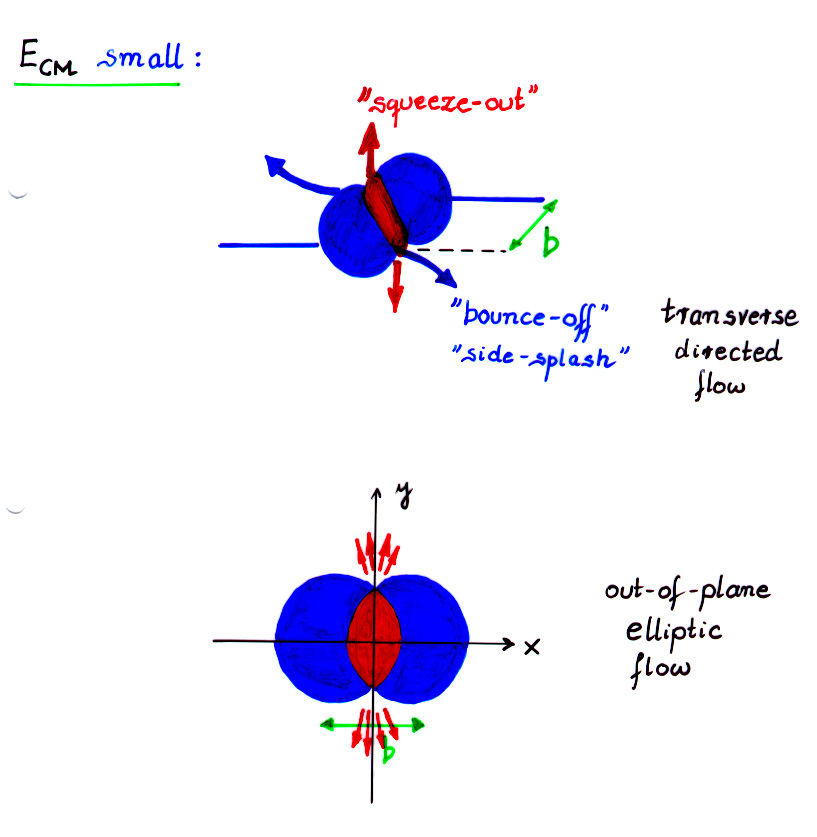
\includegraphics[width=0.75\linewidth]{images/bounce_off.jpg}
    \caption{Схематичное изображение механизмов рождения направленного (bounce-off) эллиптического (squeeze-out) потоков.}
    \label{fig:bounce_off}
\end{center}
\end{figure}
%

Партисипанты, или нуклоны сталкиващихся ядер, претерпевают многократные рассеяния.
В результате рождаются новые частицы и изменяются импульсы частиц, составляющих материю в области перекрытия.
Если время взаимодействия достаточно велико, то материю в области перекрытия можно описать при помощи статистических величин: средняя плотность, средняя температура и т.д..
При многократном рассеянии частиц, составляющих материю в области перекрытия, может происходить подпороговое рождение частиц.
Сравнивая коллективные потоки различных типов частиц, рожденных в области перекрытия можно судить о степени термализации или релаксации энергии в области перекрытия.
Чем ближе потоки различных типов сталкивающихся частиц к среднему значению, тем больше степень термализации материи.
По степени термализации можно судить о времени существования материии в области перекрытия.  

Реакция и развитие коллективных эффектов останавливаются на стадии столкновения, обычно называемой фриз-аут. 
В этой фазе плотности достаточно малы, чтобы в течение типичной длины пролета больше не происходило взаимодействия.
Хотя многие наблюдаемые (например, спектры рожденных частиц) теряют память о начальных условиях во время процесса эволюции, ожидается, что коллективные потоки адронов несут информацию о самых ранних этапах столкновения~\cite{Herrmann:1999wu}.
Коллективные потоки рожденных адронов сильно зависят от начальной геометрии столкновения.
Коллективное движение рожденых адронов обусловлено взаимодействием частиц составляющих материю в области перекрытия.
Характер этого взаимодействия обусловлен свойствами материи, которые описываются уравнением состояния.
Поэтому зная изначальную геометрию столкновения, которая определяется центральностью и измеряя итоговую анизотропию рожденных частиц можно извлечь уравнение состояния сильновзаимодействующей материи.

Коллективное движение частиц приводит к корреляции импульсов рожденных адронов.
Таким образом, изучая эту корреляцию, можно количественно оценить коллективные эффекты.
Однако это не единственный канал, по которому импульсы рожденных частиц могут быть скоррелированы.
К примеру, импульсы частиц, рожденных в слабом или сильном распаде резонанса относятся следующим образом:
%
\begin{equation}
    P = P_1 + P_2,
\end{equation}
где $P$ --- 4-импульс резонанса, $P_{1,2}$ --- импульсы рожденных в распаде частиц.
Также в силу сохранения поперечного (полного) импульса системы справедливо следующее соотношение:
%
\begin{equation}
    \sum_{k=1}^{N} \vec{p_T}^k = 0,
\end{equation}
где $N$ --- множественность рожденных частиц, $\vec{p_{T}}^k$ --- поперечный импульс $k$-й частицы.
Корреляция импульсов частиц, рожденной в бинарном столкновении частиц, составляющих материю тоже подчиняется законам сохранения импульса:
%
\begin{equation}
    P_1 + P_2 = P_3 + P_4 + P_5.
\end{equation}

Описанные выше эффекты не имеют отношения к коллективному движению частиц, однако обеспечивают корреляцию импульсов.
Такие эффекты носят название непотоковых корреляций и осложняют измерение коллективных эффектов.
Поэтому для подавления непотоковых эффектов чаще всего рассматривается корреляция большого колличества частиц.
Также для подавления корреляций не связанных с коллективным движением частиц можно рассматривать корреляцию областей со значительнми разделением по кинематике.
Оценка вклада остаточных непотоковых корреляций является важной задачей при измерении коллективных эффектов.

\subsection{Определение уравнения состояния сильновзаимодействующей материи}

Уравнение состояния сильновзаимодействующей материи можно восстановить путём сравнения экспериментально наблюдаемых сигналов, доступных из столкновения тяжелых ионов (таких как выходы частиц, их импульсные спектры, коллективная анизотропия рожденных частиц) с предсказаниями теоретических моделей с различными EOS.
Прямые вычисления КХД возможны лишь при нулевых бариохимических потенциалах и в области больших чистых барионных плотностей неприменимы.
Поэтому теоретические модели в области низких энергий столкновений ограничены описанием динамики системы.
Можно выделить два вида динамических моделей: релятивистская гидродинамика~\cite{Stoecker:1986ci,Hung:1994eq,Werner:2010aa} и транспортные модели, основанные на релятивистском транспортном уравнении Больцмана~\cite{Molnar:2004yh,Xu:2004mz}.

Первый подход основан на приближении, что образованная система может быть описана как расширяющаяся жидкость, достигшая локального термодинамического равновесия. 
Основное преимущество такого подхода заключается в довольно лёгкой интерпретации уравнения состояния системы, которое вычисляется в термодинамическом подходе~\cite{Stoecker:1986ci}.
Основная проблема релятивистской гидродинамики заключается в предположении, что система успевает достичь термодинамического равновесия, что может быть неверно.

Транспортные модели лишены этого недостатка, поскольку описывают процесс столкновения ядер через многократные упругие и неупругие рассеяния адронов.
Наличие или отсутствие локального равновесия не влияет на решение релятивистского транспортного уравнения Больцмана.
Недостатком же такого подхода является то, что он основан на предположении, что многочастичные рассеяния можно свести к двухчастичным.
До сих пор, справедливо ли это предположение, не доказано.
Более того, для моделирования каждого вида рассеяния необходимо обладать значениями сечений взаимодействий, которые для тяжелых резонансов остаются свободными параметрами модели.
Имплементация уравнения состояния системы часто выполняется путём варьирования среднего потенциала взаимодействия~\cite{Nara:2016hbg}.

Транспортные модели описывают распространение частиц в образованной материи при помощи одночастичного потенциала $U(\rho, p)$, где $\rho$ и $p$ --- плотность материи достигнутая в столкновении и импульс частицы.
Этот потенциал в простейшем виде можно выразить в виде параметризации Скёрма без импульсной зависимости:
\begin{equation}
    U(\rho) = a(\rho/\rho_0) + b(\rho/\rho_0)^\sigma
    \label{eq:skyrme}
\end{equation}
Параметры $a$, $b$ и $\sigma$ подбираются таким образом, чтобы отвечать свойствам системы: энергия связи на нуклон плотность насыщения и несжимаемость материи K.
Несжимаемость материи в ядерной физике определяется следующим образом:
\begin{equation}
    K = R^2 \frac{d^2 e/\rho}{ d^2 R },
\end{equation}
где вторая производная берётся в предположении постоянного числа нуклонов и энтропии, $e$ --- плотность энергии и $R$ --- радиус ядра.
Предполагается, что коллективное расширение области перекрытия чувствительно к коэффициенту несжимаемости материи $K$.

Сравнение теоретических предсказаний с потенциалом~(\ref{eq:skyrme}) для среднего импульса $\langle p_x / A \rangle$ с экспериментальными данными показывает лучшее согласие для очень больших значений $K \ge 380$~MeV~\cite{Kruse:1985hy, Molitoris:1985gs}.
В то же самое время феноменологический подход с импульсно-зависимым потенциалом, описанный в~\cite{Gale:1987zz, Aichelin:1987ti, Welke:1988zz, Haddad:1995vt} показывает хорошее согласие с данными при относительно небольшой несжимаемости $K=215$~МэВ.
Хотя теоретические модели с импульсно-зависимым потенциалом $U(\rho, p)$ довольно хорошо описывают равновесные свойства ядерной материи, они могут довольно сильно различаться между собой в неравновесной фазе столкновения, которая доминирует в начальные моменты реакции.
Это может влиять на более поздние этапы столкновения и приводить к различной достигнутой плотности.

При таком динамическом подходе, параметры уравнения состояния ядерной материи быстро меняются со временем, а все наблюдаемые являются наблюдаемыми конечного состояния. 
Экспериментально недоступны ни начальное ни промежуточные состояния. 
При энергиях столкновения $E_{kin}<10A$~ГэВ время расширения материи в области перекрытия, которое определяется скоростью звука, сравнимо со временем пролёта сталкивающихся ядер.
Поэтому спектаторы --- остатки сталкивающихся ядер --- блокируют вылет рожденных частиц в плоскости реакции, что приводит к отрицательному $v_2$ рожденных частиц. 
Смешивание холодной спектаторной и горячей, рожденной в столкновении материй и расширение этой материи приводят к положительным значениям $v_1$ протонов.
Уменьшение времени пролёта при увеличении энергии столкновения, приводит к спаду магнитуды направленного и эллиптического потоков. 
С ростом энергии эллиптический поток меняет знак с отрицательного на положительный, что свидетельствует о преимущественном вылете частиц в плоскости реакции.
Система, образованная в столкновения тяжелых ионов в данной области энергии характеризуется сложной геометрией из-за присутствия спектаторов.
Изучение зависимости коллективных потоков от геометрии столкновения и размеров системы может пролить свет на свойства созданной в столкновении материи.

Экспериментальные измерения направленного потока протонов в диапазоне энергий 2-10$A$~Гэв были выполнены коллаборацией E895 на ускорителе AGS в Национальной Лаборатории в Брукхевене~\cite{E895:2000maf}. 
Теоретический анализ этих измерений был выполнен Данилевичем, Лейси и Линчем в 2002 году~\cite{Danielewicz:2002pu}.
Экспериментальные данные для наклона бокового потока и эллиптического потока были сопоставлены с теоретическими предсказаниями для различных коэффициентов несжимаемости материи $K$.
Сравнение показано на рис.~\ref{fig:Danilewicz}. 
Экспериментальные данные позволили отсечь лишь экстремальные значения коэффициента несжимаемости $K$.
Значения для наклона бокового потока $F$ лучше согласуются с теоретическими предсказаниями с $K=210$~МэВ. 
Данные для эллиптического потока лучше описываются более жестким уравнением состояния с $K=300$~МэВ.
Это несоответствие может быть вызвано вкладом корреляций, не связанных с коллективным движением рожденных адронов (непотоковые корреляции).
Новые экспериментальные данные, выполненные методами, позволяющими учесть вклад непотоковых корреляций позволят разрешить эту неоднозначность полученных значений $K$.

\begin{figure}[h]
    \centering
    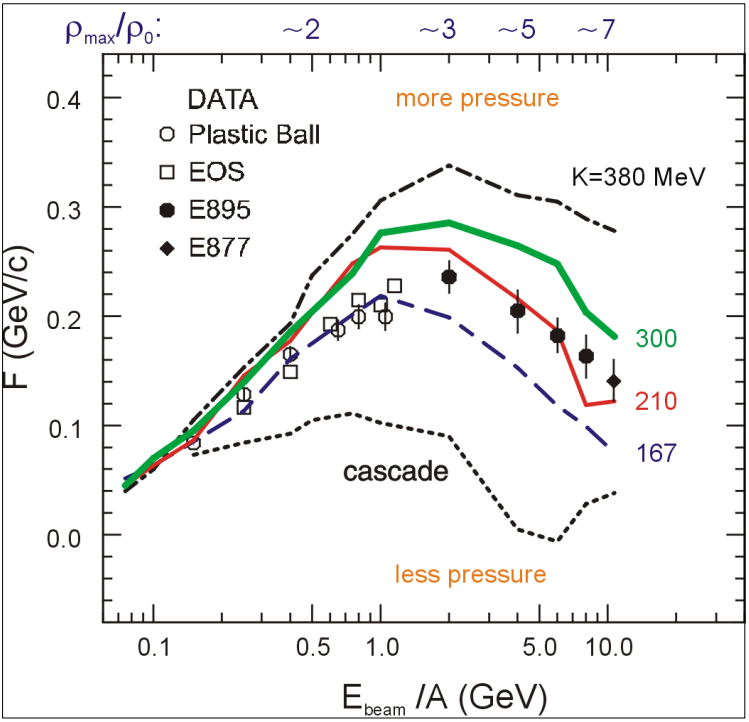
\includegraphics[width=0.45\linewidth]{images/Danilewicz_F_energy.png}
    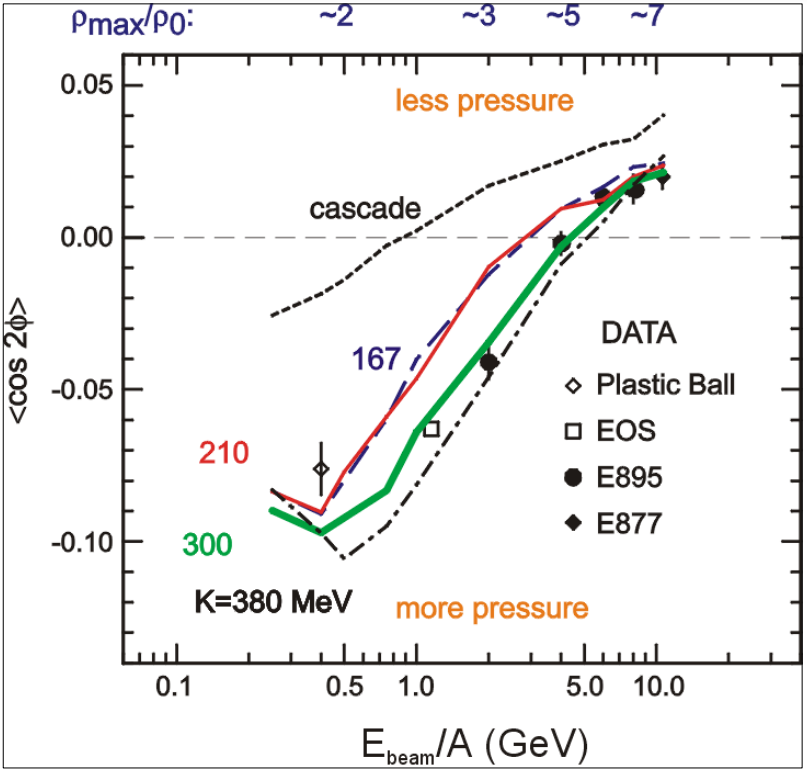
\includegraphics[width=0.45\linewidth]{images/Danilewicz_Elliptic_energy.png}
    \caption{Сравнение данных для наклона бокового потока (слева) и эллиптического потока (справа) как функция энергии с теоретическими расчетами для разных значений коэффициента несжимаемости~\cite{Danielewicz:2002pu}.}
    \label{fig:Danilewicz}
\end{figure}

На рис.~\ref{fig:dv1dy_energy} представлена зависимость наклона направленного потока протонов $dv_1/dy|_{y=0}$ от энергии столкновения ядер золота.
На рисунке показаны данные с экспериментов FOPI~\cite{FOPI:2011aa} и предварительные данные эксперимента STAR Fixed Target.
Наблюдается монотонное уменьшение наклона с ростом энергии.
Новые экспериментальные измерения направленного потока позволят дополнить существующие мировые данные по коллективным потокам протонов в области энергии в несколько $A$~ГэВ.
%
\begin{figure}
    \centering
    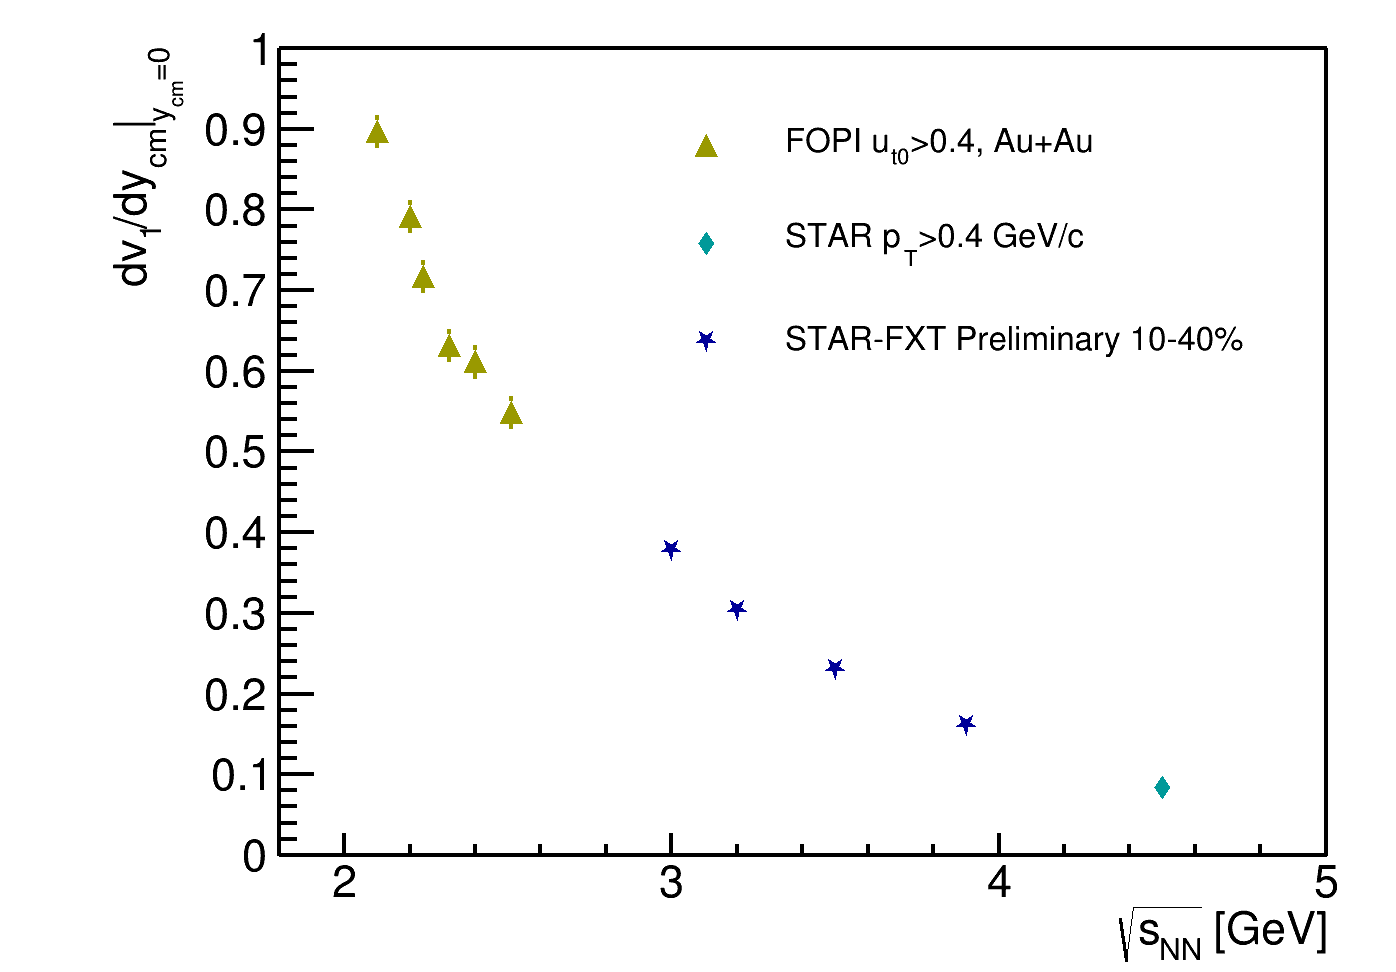
\includegraphics[width=0.5\linewidth]{images/dv1dy_sqrt_snn.png}
    \caption{Зависимость наклона направленного потока протонов $dv_1/dy|_{y=0}$ от энергии столкновения ядер золота.}
    \label{fig:dv1dy_energy}
\end{figure}

\section{Основные определения}

\subsection{Центральность столкновения}
\label{theory:centrality}
Наблюдаемые, чувствительные к свойствам созданной в области перекрытия материи, зависят от геометрии столкновения~\cite{ALICE:2010mlf,ALICE:2015juo}.
Геометрия столкновения может быть описана при помощи таких переменных, как прицельный параметр столкновения $b$, число бинарных нуклон-нуклонных столкновений $N_{col}$ и число нуклонов-участников взаимодействия $N_{part}$.
Для того, чтобы характеризовать геометрию столкновения наименее зависящим от экспериментальной установки методом, была введена такая величина, как центральность столкновения $C_b$.
Центральность столкновения определяется как доля полного сечения взаимодействия сталкивающихся ядер $\sigma_{inel}^{AA}$ при данном значении прицельного параметра $b$:
\begin{equation}
    C_b = \frac{1}{\sigma_{inel}^{AA}} \int_{0}^{b} \frac{d\sigma}{db'}db',
\end{equation}
где $d\sigma/db$ --- дифференциальное сечение взаимодействия ядер.

Прицельный параметр $b$ не может быть измерен, поэтому для определения центральности в условиях эксперимента используются скоррелированные с ним величины, такие как например множественность рожденных частиц~\cite{Segal:2020ftt,HADES:2017def}.
Центральность по множественности столкновения определяется формулой:
\begin{equation}
    C_M = \frac{1}{\sigma_{inel}^{AA}} \int_{M}^{\infty} \frac{d\sigma}{dM'}dM',
\end{equation}
где $M$ --- множественность зарегистрированных рожденных частиц.

Столкновения ионов группируются в классы центральности, согласно множественности рожденных частиц.
Поскольку в распределении прицельного параметра и числа рожденных частиц, наблюдается не нулевая ширина, определеные классы центральности по множественности лишь в среднем совпадают с определенными по прицельному параметру.
События с классом центральности 0\% отвечают наиболее центральным столкновениям и 100\% --- наиболее переферическим.

Для вычисления значений прицельного параметра (или других геометрических параметров) в определенных по множественности классах центральности, часто использутся модель Монте-Карло Глаубера~\cite{Miller:2007ri}.
Модель Монте-Карло Глаубера описывает столкновения ядер следующим образом:
\begin{itemize}
    \item Столкновения ионов рассматривается как последовательность независимых нуклон-нуклонных столкновений, вероятность которых определятся сечением неупругих нуклон-нуклонных рассеяний.
    \item Изначальное распределение нуклонв в ядре разыгрывается при помощи метода Монте-Карло согласно распределению Вудса-Саксона ядерной плоности:
    \begin{equation}
        \rho(r) = \frac{ \rho_0 }{ 1 + e^{ (r-R)/a } },
        \label{ eq:woods_saxon }
    \end{equation}
    где $\rho_0$ --- нормировочный коэффициент, $r$ --- расстояние от центра ядра, $R$ --- радиус ядра и $a$ --- параметр толщины оболочки.
    Данные параметры подбираются для каждого ядра и каждой энергии столкновения.
    \item Каждый нуклон движется по прямолинейной траектории во время процесса столкновения.
\end{itemize}

Множественность столкновения моделируется при помощи геометрических параметров ($N_{part}$, $N_{col}$), разыгранных в модели МК-Глаубера.
Суммарная множественность набирается из множественности частиц, рожденных в каждом единичном источнике $a$: $M=\sum_{a=1}^{N_a} M_a$, где $N_a$ --- число источников.
Число источников определятся формулой, которая моделирует жесткие процессы через зависимость от $N_{col}$ и мягкие процессы через зависимость от $N_{part}$:
\begin{equation}
    N_a = f N_{part} + (1-f) N_{col}.
\end{equation}

Для каждого источника $a$ число рожденных частиц $M_a$ разыгрывается при помощи отрицательного биномиального распределения с параметрами $\mu$ --- среднее и $k$ --- ширина:
\begin{equation}
    P_{\mu,k}(n) = \frac{ \Gamma (n+k) }{ \Gamma(n+1) \Gamma(k) } \frac{ (\mu/k)^n }{ (\mu/k+1)^{n+k} },
\end{equation}
где $P_{\mu,k}(n)$ --- вероятность источника родить $n$ частиц.

В дальнейшем параметры $f$, $\mu$ и $k$ подбираются таким образом, чтобы разыгранная множественность наилучшим образом описывала экспериментальное распределение множественности.

\subsection{Вектора потоков $u_n$ и $Q_n$}

Методы измерения коллективных потоков довольно просто описать в терминах векторов.
Для измерения азимутальных потоков каждой частице ставится в соответствие единичный вектор $u_n$ в плоскости перпендикулярной оси пучка на основании импульса частицы:
%
\begin{equation}
    \vec{u}_n = (x_n, y_n) = ( \cos n \varphi, \sin n \varphi ),
\end{equation}
%
где $\varphi$ --- азимутальный угол частицы, $n$ --- порядок гармоники. 
При очень большом количестве частиц в одном событии ($N \gg 1$), сумму по всем частицам можно заменить на интеграл (аналогично, при небольшой множественности частиц и большом числе событий, можно рассматривать все события с выбранной плоскостью реакции $\Psi^R$):
%
\begin{equation}
    \sum_{k=1}^{N} \vec{u}_n = \int_{-\pi}^{\pi} \vec{u}_n(\phi) \rho(\phi-\Psi^R) d\phi
\end{equation}
Рассмотрим интеграл по $x$-компоненте $u_n$ вектора:
%
\begin{equation}
    \int_{-\pi}^{\pi} x_n \rho(\phi-\Psi^R) d\phi =
    \int_{-\pi}^{\pi} \cos n ( \phi - \Psi^R + \Psi^R ) \rho(\phi - \Psi^R) = V_n \cos (n\Psi^R), 
\end{equation}
где $V_n$ пропорционален множественности частиц $N$ и значению $v_n$ для данной группы частиц в данном событии.
Аналогичные преобразования можно выполнить и для $y$-компоненты $u_n$-вектора, получив $V_n\sin(n\Psi^R)$.
Таким образом, сумма $u_n$-векторов в одном событии даёт оценку плоскости реакции события.

Эта оцнека, определяемая суммой единичных векторов частиц носит название $Q_n$-вектора:
%
\begin{equation}
    \vec{Q}_n = \frac{1}{C} \sum_{k=1}^{N} w_k u_n^k = \frac{|Q_n|}{C} (\cos{(n\Psi_n)}, \sin{(n\Psi_n)}),
\end{equation}
%
где $k$ --- индекс частицы в группе, $w_k$ --- вес $k$-го вектора, $N$ --- множественность частиц в группе, $\Psi_n$ --- угол плоскости симметрии данного события и данной гармоники $n$, $|Q_n|$ --- модуь $Q_n$-вектора и $C$ --- нормировочный коэффициент. 
Чем больше число частиц в событии $N$, тем ближе оценка угла плоскости симметрии к реальной ориентации плоскости реакции:
%
\begin{equation}
    \lim_{N \xrightarrow{} \infty} \frac{1}{C} \sum_{k=1}^{N} w_k u_n^k = \frac{|Q_n|}{C} (\cos (n\Psi^R), \sin (n\Psi^R) ) .
\end{equation}

\section{Методы измерения коллективной анизотропии в столкновениях тяжелых ионов}

\subsection{Методы плоскости события и скалярного произведеления}

Выбор значения нормировочного коэффициента определяет метод измерения направленного потока. 
В работе исследуются два метода: плоскости события (EP) и скалярного произведения (SP)~\cite{Mamaev:2020lpi}. 

Метод плоскости события требует такую нормировку, чтобы модуль каждого $Q_1$-вектора был равен 1, что соответствует $C=|Q_n|$. 
В работах~\cite{Borghini:2001vi, Bhalerao:2006tp} было показано, что в таком случае, измеренное значение потока $v_n\{EP\}$ нелинейно зависит от множественности частиц, использованных для вычисления $Q_n$-вектора, а также от значения самого потока. 
В пределе большого количества частиц и большого значения потока ($v_n \sqrt{M} \gg 1$), измеренные значения стремятся к среднему значению $v_n$: $v_n\{EP\} \xrightarrow{} \langle v_n \rangle$. 
В случае малого числа частиц, использованных для построения $Q_n$-вектора, а также малых значениях потока ($v_n \sqrt{M} \ll 1$), измерения стремятся к корню среднего квадрата $ v_n\{EP\} \xrightarrow{} \sqrt{ \langle v_n^2 \rangle }$.
Экспериментально измеренные значения $v_1\{EP\}$ находятся между двумя пределами: $ \langle v_n \rangle \leq v_n\{EP\} \leq \sqrt{ \langle v_n^2 \rangle } $.
В зависимости от реального значения $v_n$ (который определяется энергией столкновения и размером сталкивающихся ядер) и множественности частиц (которая зависит от энергии, размера ядер и аксептанса установки), измеренные значения $v_n\{EP\}$ могут лежать ближе к правому или левому пределам.

Второй метод, скалярного произведения (SP), требует нормировку на сумму весов $C=\sum_{k=1}^N w_k$.
Модуль $Q_n$-вектора сохраняет информацию о множественности частиц, использованных для его построения, а также их $v_n$: $|Q_n| \propto v_n M$.
Использование такой нормировки дает значения $v_n\{SP\} \xrightarrow{} \sqrt{\langle v_n^2 \rangle}$ независимо от измеренной множественности частиц, а также их $v_n$.

Несмотря на известные недостатки метода плоскости события, он до сих пор активно используется, поскольку более прост в реализации. 
В частности, измерения коэффициентов коллективных потоков $v_n$ в коллаборации HADES~\cite{HADES:2020lob} были выполнены методом плоскости события. 
В работе была произведена оценка систематической ошибки на измереные $v_n$, путём сравнения результатов полученных методами скалярного произведения и плоскости события~\cite{Mamaev:2020lpi}.

\subsection{Разрешение плоскости симметрии}

Экспериментально направленный поток можно определить как проекцию $u_n$-вектора частиц на плоскость симметрии события:
%
\begin{equation}
    v_n' =  \langle u_n Q_n \rangle = 
    V_n \langle \cos (n\phi) \cos (n\Psi_n) \rangle + V_n \langle \sin(n\phi) \sin(n\Psi_n) \rangle,
\end{equation}
%
где диагональные члены равны нулю в силу симметрии столкновения относительно плоскости реакции, а коэффициент $V_n$ появляется после усреднения модулей вектора $Q_n$.
Раскрывая тригонометрические выражения в угловых скобках, можно получить:
%
\begin{equation}
\begin{align}
    \langle \cos (n\phi) \cos (n\Psi_n) \rangle = \langle \cos n ( \phi - \Psi_n ) \rangle = 
    = \langle \cos n ( \phi - \Psi_n + \Psi^R - \Psi^R ) \rangle = \\
    \langle \cos n ( \phi - \Psi^R ) \cos n (\Psi_n - \Psi^R ) \rangle
\end{align}
\end{equation}
%
Аналогичные преобразования можно выполнить и для синусов. 
Измеренные значения направленного потока имеют вид:
%
\begin{equation}
    v_n' =  \langle u_n Q_n \rangle = 
    V_n \langle \cos n ( \phi - \Psi_n ) \cos n (\Psi_n - \Psi^R) \rangle.
    \label{eq:uq_transformation}
\end{equation}
%

Поскольку вычисленная плоскость симметрии столкновения $\Psi_n$ лишь приблизительно описывает ориентацию плоскости реакции $\Psi^R$, значение $ \langle \cos(\Psi_n - \Psi^R) \rangle \ne 1 $.
Флуктуации распределения энергии в сталкивающихся ядрах приводят к флуктуации плоскости симметрии относительно плоскости реакции реакции, как показано на рис.~\ref{fig:pp_sp_rp}
Поэтому измеренные значения $v_n'$ будут отличаться от действительных.
Для коррекции этого этого эффекта, необходимо ввести поправочный коэффициент разрешения:
%
\begin{equation}
    R_n = V_n \langle \cos n (\Psi_n - \Psi^R) \rangle.
\end{equation}
%

%
\begin{figure}[ht]
\begin{center}
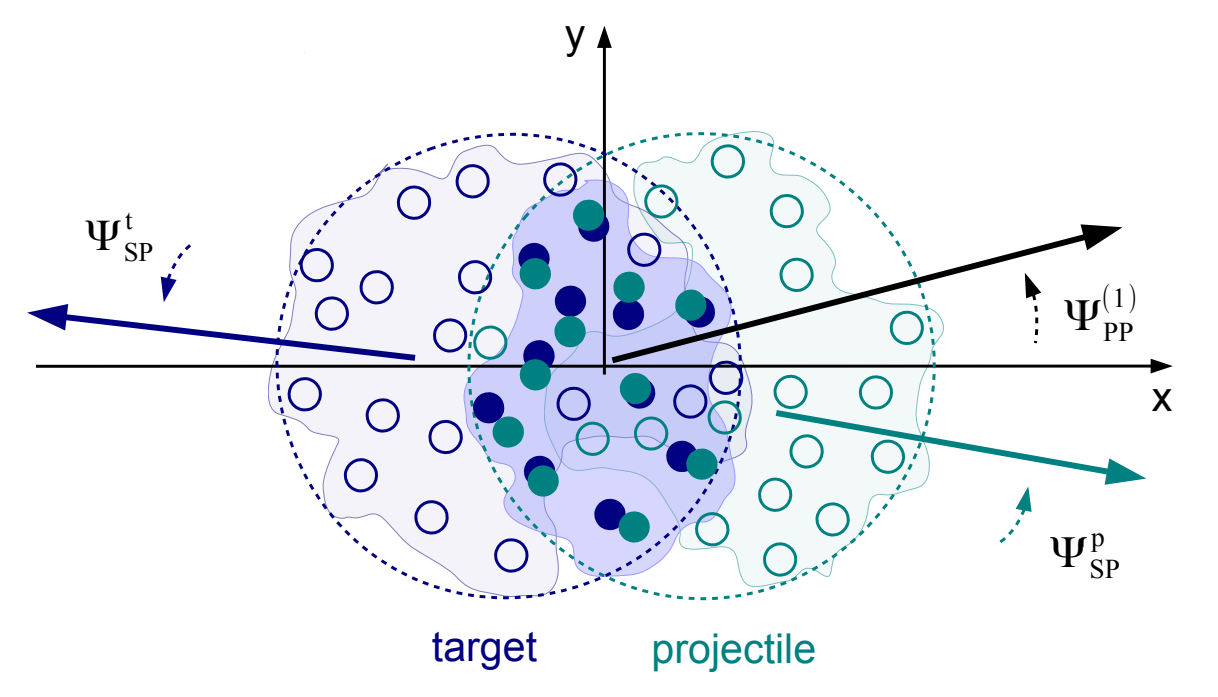
\includegraphics[width=0.75\linewidth]{images/v1_pp_sp.png}
\caption{Схематическое представление сталкивающихся ядера в плоскости перпендикулярной направлению пучка.}
\label{fig:pp_sp_rp}
\end{center}
\end{figure}
%

Скорректированные на разрешение значения $v_1$ могут быть записаны следующим образом: 
%
\begin{equation}
    v_n =  \frac{ \langle u_n Q_n \rangle }{R_n},
    \label{eq:v1_formula}
\end{equation}
%

\subsection{Метод случайных подсобытий}

Для вычисления $R_n$ в эксперименте, можно воспользоваться попарными корреляциями $Q_n$-векторов (преобразование выполнено аналогично уравнению (\ref{eq:uq_transformation})): 
%
\begin{equation}
    \langle Q_n^a Q_n^b \rangle = V^a_n V^b_n \langle \cos n (\Psi^a_n - \Psi^R) \cos(\Psi^b_n - \Psi^R) \rangle,
\end{equation}
%
где индексами $a$ и $b$ обозначены две различных группы частиц, в каждой из которых $Q_n$-вектор вычислялся независимо.

Наиболее простым методом вычисления разрешения является метод двух подсобытий:
%
\begin{equation}
    R_n\{a,b\} = \sqrt{ \langle Q_n^a Q_n^b \rangle } = \sqrt{ V_n^2 \langle \cos^{2}( \Psi^{a,b}_n - \Psi_R ) \rangle },
\end{equation}
где индексами $a$ и $b$ обозначены две группы частиц, идентичные по множественности и значению $v_n$, в которых $Q_n$-вектор вычислялся независимо.
В коллайдерных экспериментах, где аксептанс часто симметричен относительно средних быстрот, в качестве подсобытий $a$ и $b$ могут быть выбраны частицы в диапазонах по быстроте, симметричных относительно нуля.
В экспериментах с фиксированной мишенью, где такое выполнить невозможно в силу несимметричного аксептанса, иногда пользуются методом, называемым метод случайных подсобытий.
Подсобытия $a$ и $b$ набираются случайным образом из частиц в выбранном кинематическом окне.
Этот метод прост в исполнении, однако корреляция $Q_1$-векторов из одной кинематической области может быть подвержена довольно большому вкладу непотоковых корреляций~\cite{Mamaev:2020lpi}.
Экспериментальные значения $v_n$, полученные коллаборацией HADES~\cite{HADES:2020lob} измерены, испльзуя метод случайных подсобытий для коррекции на разрешение плоскости симметрии. 
Вычисляя $R_n$ отличным от использованного коллаборацией HADES методом, предлагается оценить вклад непотоковых корреляций в измерененные значения $v_n$~\cite{Mamaev:2020lpi, Mamaev:2020qom}.

\subsection{Метод трех подсобытий}

Комбинируя различные попарные корреляции векторов, можно вычислить разрешение плоскости симметрии для данного $Q_n$-вектора:
%
\begin{equation}
    R_n\{a(b,c)\}  =  \sqrt { \frac{ \langle Q_n^a Q_n^b \rangle \langle Q_n^a Q_n^c \rangle }{ \langle Q_n^b Q_n^c \rangle} },
\end{equation}
%
где $a$, $b$ и $c$ --- три различных группы частиц, в каждой из которых $Q_1$-вектор вычислялся независимо.
Этот метод вычисления $R_n$ носит название метод трёх подсобытий.
Метод трёх подсобытий не накладывает ограничений на множественность частиц в каждой группе, что даёт большую свободу в выборе кинематических диапазонов для определения $Q_n$.
Корреляции $Q_n$, рассчитанных в близких кинематических диапазонах, всё еще могут быть подвержены непотоковым эффектам.
Это может приводить к неверному рассчету значений поправочного коэффициента $R_n$.
Автором предлагается исследовать связанную с этим систематическую ошибку путем сравнения $R_n$, полученнного с использованием различных комбинаций $Q_1$ (к примеру $R_1\{a(b,c)\}$ и $R_1\{a(b,d)\}$).
Эффекты не связанные с коллективным движением частиц могут вносить вклад в корреляцию между $u_n$-векторами частиц и $Q_n$-векторами плоскости симметрии.
Сравнивая $v_n$, полученные относительно различных плоскостей симметрии (к примеру, $v_n\{a\}$ и $v_n\{b\}$), предлагается вычислить вклад непотоковых корреляций в результаты для коллективного потока~\cite{Mamaev:2020qom,Mamaev:2023fpr,Mamaev:2023yhz,Mamaev:2024}. 

\section{Эффекты, необходимые учитывать при измерени коллективной анизотропии}

\subsection{Влияние эффективности на измеренный $v_n$}

Коллективная анизотропия рожденных в столкновении частиц обычно измеряется дифференциально как функция центральности, поперечного импульса и быстроты.
Неоднородная эффективность детектора в зависимости от этих переменных может приводить к неправильным значениям потоков при усреднении по этим переменным.
К примеру, при усреднении коэффициентов потока по поперечному импульсу в границах $p_T^{1,2}$ вклад неоднородной эффективность детектора $e(p_T)$ можно выразить следующим образом:
\begin{equation}
    v_n(p_T^1, p_T^2) = \int_{p_T^2}^{p_T^2} dp_T \frac{dN}{dp_T} e(p_T) v_n(p_T),
\end{equation}
где $\frac{dN}{dp_T}$ --- распределение частиц по поперечному импульсу.
Измеренные значения $v_n(p_T^1, p_T^2)$ будут отличаться от настоящего среднего в данном диапазоне импульсов.

Для коррекции на этот эффект, обычно вычисляется карта эффективности $e(p_T, y)$ установки при помощи Монте-Карло моделирования отклика детектора.
И усреднение по поперечному импульсу и быстроте выполняется с весом, обратным эффективности $1/e(p_T, y)$.

\subsection{Влияние азимутальной неоднородности аксептанса детектора}

Значительный вклад в результаты измерения азимутальных потоков может вносить неоднородность аксептанса детектора. 
Азимутальная анизотропия аксептанса искажает распределение $u_n$  и $Q_n$-векторов, которые в идеальном случае должны быть равномерными. 
Для коррекции этого эффекта был использован метод, описаный в работе~\cite{Selyuzhenkov:2007zi}.
Поскольку плоскость реакции распределена равномерно, в пределах большого количества столкновений формулу~(\ref{eq:v1_formula}) можно преобразовать следующим образом:
%
\begin{equation}
    v_n =  2\frac{ \langle x_n X_n \rangle }{R_n^X} = 2\frac{ \langle y_n Y_n \rangle }{R_n^Y},
    \label{eq:v1_formula}
\end{equation}
%
где $x_n$ и $y_n$ --- компоненты $u_n$-вектора, $X_n$ и $Y_n$ --- компоненты $Q_n$-вектора и $R_n^{X,Y}$ --- разрешение плоскости симметрии, вычисленное при помощи корреляций компонент $Q_n$-векторов.
Азимутальная неоднородность детектора нарушает это равенство.

Основные эффекты, вызываемые неоднородностью аксептанса могут быть выражены в следующем:
\begin{enumerate}
    \item Сдвиг $u_1$ ($Q_1$) вектора из-за ненулевых средних значений компонент:
    \begin{equation}
        \langle x_1 \rangle \ne 0, \langle y_1 \rangle \ne 0
    \end{equation}
    Коррекция на этот эффект носит название перецентровки.
    \item Поворот $u_1$ ($Q_1$) векторов. Коррекция на этот эффект называется коррекцией поворота
    \item Сужение/Расширение распределения компонент $u_1$ ($Q_1$) вектора. Коррекция носит название ремасштабирования.
\end{enumerate}
Схематическое представление эффекта применения коррекций представлено на рис.~\ref{fig:qn_corrections}.

\begin{figure}[h]
    \centering
    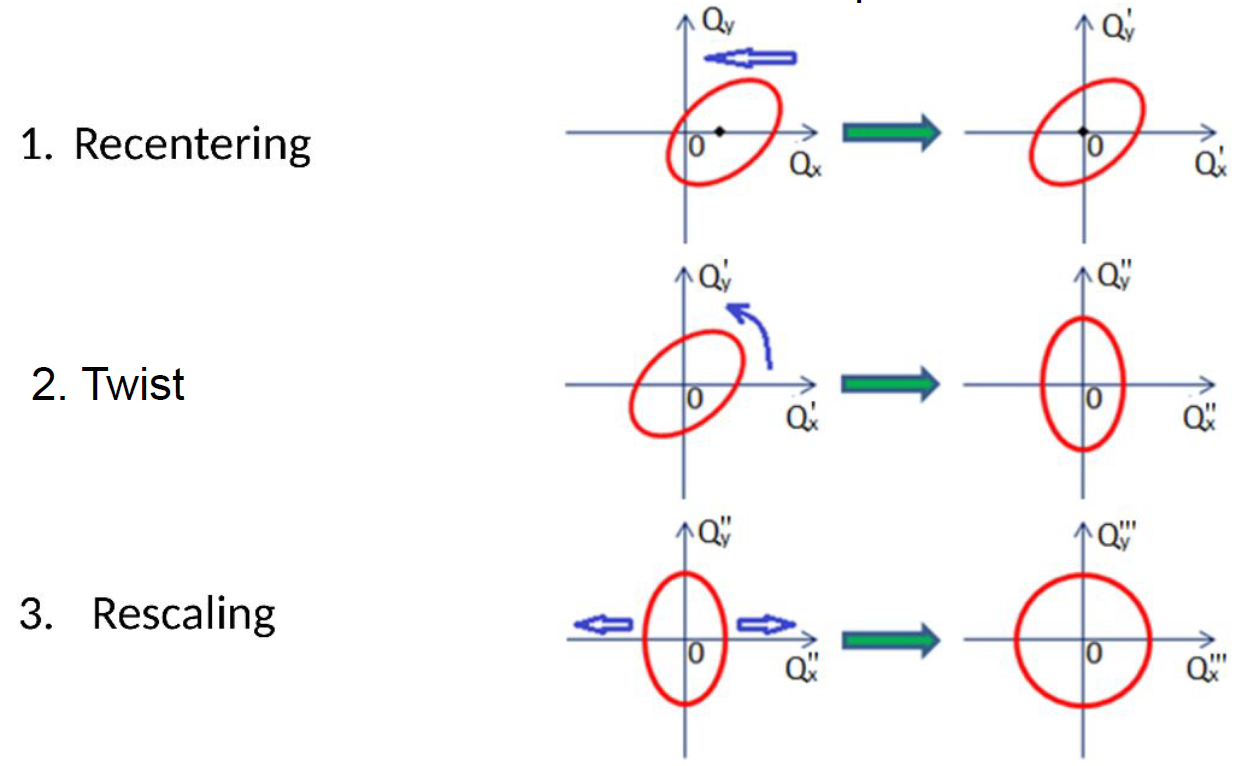
\includegraphics[width=0.5\linewidth]{images/corrections_for_nonuniformity.png}
    \caption{Схематическое представление эффекта применения каждого этапа коррекций, описанных в~\cite{Selyuzhenkov:2007zi}.}
    \label{fig:qn_corrections}
\end{figure}
Ранее описанные выше методы коррекции применялись лишь на коллайдерных экспериментах с относительно однородным аксептансом. 
Впервые коррекции рецентровки, поворота и ремасштабирования будут применятся автором для коррекции сильно неоднородного аксептанса установок HADES и BM@N.
Систематический вклад остаточной азимутальной неоднородности аксептанса детектора предлагается оцененить путём сравнением результатов полученных с использованием различных компонент $u_1$ и $Q_1$-векторов~\cite{Mamaev:2020qom,Mamaev:2023yhz}. 

\subsection{Вычисление $Q_1$ при помощи модульных детекторов}

В данной работе для восстановления плоскости симметрии используются фрагменты ядра, которые взаимодействовали с областью перекрытия лишь упруго (спектаторы). 
Спектаторные фрагменты отталкиваются областью перекрытия в плоскости реакции (см.~\ref{fig:pp_sp_rp}), поэтому могут быть использованы для реконструкции плоскости симметрии. 
Часто в экспериментах по столкновению тяжёлых ионов регистрация спектаторных частиц выполняется при помощи передних детекторов, имеющих модульную структуру. 
В таком случае $Q_n$-вектор будет определяться суммарной азимутальной анизотропией распределения сигнала по модулям:
%
\begin{equation}
    \vec{Q}_n  = \frac{1}{C} \sum_{k=1}^M w_k ( \cos n \varphi, \sin n \varphi ),
\end{equation}
%
где $k$ --- индекс модуля, $M$ --- число модулей, использованных в построении $Q_n$-вектора, $w_k$ --- сигнал в данном модуле, $\varphi$ --- азимутальный угол данного модуля. 
Нормировочный коэффициент $C$ может также принимать значения $C=|Q_1|$ (метод плоскости события) или $C=\sum_{k=1}^M w_k$ (метод скалярного произведения).
Взвешивание на сигнал в данном модуле необходимо, поскольку в один и тот же модуль могут попасть более одной частицы.
Корреляции между $Q_n$-векторами, определёнными из разных групп модулей одного детектора также могут быть подвержены непотоковым корреляциям.
К примеру, между соседними модулями может происходить перетекание сигнала вследствие конструкционных особенностей детектора (например, в адронных калориметрах присутствует поперечное распространение ливней).
Также при распаде осколков сталкивающихся ядер, фрагменты могут вызвать отклик соседних модулей, что снова приведёт к корреляциям между модулями, которые не относятся к коллективному движению частиц.
Такие корреляции могут искажать значения разрешения $R_n$, полученного лишь при помощи $Q_n$-векторов из передних детекторов.
Автором предлагается дополнительно определить $Q_n$-вектора из треков рожденных частиц.
Это позволит внести значительное разделение между $Q_n$-векторами из передних детекторов и треков частиц.
Комбинируя различные группы $Q_n$-векторов, возможно оценить вклад непотоковых корреляций в значения $R_n$ для плоскостей симметрии спектаторов~\cite{Mamaev:2023fpr,Mamaev:2023yhz,Mamaev:2024}.

\section{Выводы к главе 1}

В главе был приведён обзор существующей литературы по коллективной анизотропии рожденных в столкновении частиц. 
Были описаны основные механизмы образования коллективной анизотропии и представлены обоснования необходимости ее измерения.
В главе изложены основные методы измерения коллективной анизотропии рожденных в столкновении частиц.
Определены единичный вектор частиц $u_n$ и вектор плоскости симметрии события $Q_n$.
Приведены экспериментальные методы оценки плоскости реакции и измерения коэффициентов коллективного потока $v_n$ в терминах $u_n$ и $Q_n$ векторов.
В главе обсуждаются преимущества и недостатки методов плоскости события и скалярного произведения для оценки коллективных потоков. 
Автором предлагается оценить систематическую ошибку измерения коэффциентов $v_n$ методом плоскости события, полученных коллаборацией HADES, путём сравнения со значениями, полученными методом скалярного произведения.
Описаны методы вычисления поправочного коэффициента разрешения, такие как метод случайных подсобытий и метод трёх подсобытий.
В главе обсуждается вклад непотоковых корреляций в вычисленные значеняи $R_n$ для методов случайного подсобытия и метода трёх подсобытий.
Автор диссертации предлагает сравнивать разрешение $R_n$, полученное с использованием различных комбинаций $Q_n$-векторов для оценки и минимизации вклада непотоковых корреляций в коэффициент разрешения. 
Сравнивая $v_n$, полученный относительно различных плоскостей симметрии $Q_n$ предлагается оценить систематическую ошибку для измеренных значений коллективных потоков. 
В главе обсуждается влияние неоднородности азимутального аксептанса детектора на измерения $v_n$.
Автором предлагается использовать коррекции, ранее опробованные на относительно однородном аксептансе коллайдерных установок, для устранения эффектов сильно неоднородного аксептанса экспериментов с фиксированной мишенью. 
Автор диссертации излагает особенности оценки плоскости реакции при помощи спектаторных передних детекторов, имеющих модульную структуру.
Приводится описание эффектов, влиящих на корреляцию между $Q_n$-векторами из модульных детекторов. 
Автором предлагается метод учёта этих эффектов при вычислении коэффициента разрешения $R_n$.